\chapter{Fazit}
\label{chap:closing}
% TODO: Forschungsfrage nochmal aufgreifen?
Die digitale Unterstützung der Navigation und Exploration durch augmentierte Inhalte ist ein Thema, das in der Vergangenheit bereits ausgiebig von Forschung und Industrie behandelt wurde.
Die Idee, eine augmentierte Karte als Megamap um die Nutzer herum in die Umgebung zu integrieren, ist aber bisher nur aus Videospielen wie z.\,B. \emph{Tom Clancy's The Division} bekannt.
In der vorliegenden Masterarbeit wurde untersucht, ob sich eine solche Megamap auch für die \enquote{reale} Welt umsetzen lässt.
Zu diesem Zweck wurde das Konzept einer Megamap für den Einsatz mit einem Mixed-Reality-HMD entwickelt.
Virtuelle Gebäudekarten sollen als Megamap in das reale Umfeld der Nutzer projiziert werden, sodass diese sich einen Überblick der Umgebung verschaffen können.
Verschiedene explorative Interaktionselemente aus bereits existierenden Kartenanwendungen sind in das Konzept mit eingeflossen und wurden für den Einsatz in Innenräumen neu interpretiert.
Auf Basis dieses Konzepts wurde ein erster Prototyp der Megamap für die HTC~Vive entwickelt.
In einer Nutzerstudie ($N=15$) wurde mit dem Prototyp die Nutzbarkeit, Effektivität und Effizienz der Megamap für die Suche nach Objekten und den Aufbau einer räumlichen Vorstellung der Umgebung untersucht.
Die Megamap wurde in zwei Varianten getestet (Fußboden- und Bauchhöhe).
Als Vergleichsbasis diente hierzu eine herkömmliche 2D-Darstellung der Gebäudekarten.
Die statistische Analyse der quantitativ erhobenen Daten ergab keine Vorteile der Megamap gegenüber der 2D-Variante in Bezug auf Effektivität oder Effizienz.
Für die Suche nach Objekten auf der Karte bewies sich die 2D-Darstellung als die effizientere Option mit einer ca. \SIrange{33}{36}{\percent} kürzeren Suchzeit gegenüber den Megamaps.
Weiterhin bewerteten die Probanden die Nutzbarkeit der 2D-Alternative besser als die der Megamap.
In einem kurzen Leitfadeninterview wurden zudem die subjektiven Meinungen der Probanden zu der Megamap eingeholt.

\section{Probleme des Megamap-Prototyps}
Durch die Nutzerstudie, die Interviews sowie den Erfahrungen bei der Implementierung offenbaren sich drei Probleme des aktuellen Megamap-Prototyps.
Hieraus ergeben sich Ansatzpunkte für zukünftige Verbesserungen und Erweiterungen der Megamap.

\subsection*{Fehlende Suchfunktion und andere Explorationselemente}
Der Hauptgrund für den großen Zeitunterschied zwischen der 2D-Karte und den 3D-Megamaps (siehe \autoref{ssec:searchtime}) ist das Fehlen einer Suchfunktion.
Herkömmliche Kartenapplikationen, wie z.\,B. die in \autoref{chap:concept} analysierten Webanwendungen, verfügen über eine Suchfunktion für eine spezifische und/oder offene Suche nach Zielorten.
Eine manuelle Suche auf der Karte nach Zielen ist daher nicht notwendig.
In der Nutzerstudie war allerdings die manuelle Suche nach Zielen auf der Karte gefordert.
Dies begünstigt die 2D-Variante, da im Gegensatz zur 3D-Megamap alle Ziele gleichzeitig von den Probanden zu sehen waren.
Dieser Unterschied könnte durch das Implementieren einer Suchfunktion für die Megamap ausgeglichen werden.

Aber auch andere Explorationselemente fehlen im Prototyp.
Das Megamap-Konzept aus \autoref{chap:concept} sieht eine Reihe von Elementen vor, die im aktuellen Prototyp nicht umgesetzt sind.
Dieser wurde mit dem Fokus auf die Aufgabenstellung der Nutzerstudie entwickelt und stellt somit lediglich eine begrenzte Realisierung des Konzepts dar.
Die eigentliche Kartenfunktionalität kommt dabei zu kurz.
Insofern ist die konkrete Implementierung nur teilweise repräsentativ zur Beantwortung der Forschungsfrage dieser Masterarbeit.
Gleichzeitig bedeutet dies, dass das Potential der Megamap bei Weitem nicht ausgeschöpft ist und das Konzept der Megamap für zukünftige Arbeiten weiterhin interessant bleibt.

\subsection*{Limitierung auf VR-Hardware}
Der Prototyp wurde für ein VR-HMD entwickelt, da das gewünschte MR-HMD (Magic Leap One) für die Implementierung nicht zur Verfügung stand.
Der Nachweis, dass sich die Megamap für den Einsatz in einem tatsächlichen MR-Szenario eignet, steht weiterhin aus.
Es wurde bei der Implementierung versucht, die Übertragbarkeit von dem VR-Prototyp auf MR aufrecht zu erhalten.
Dazu wird die reale Umgebung durch eine virtuelle simuliert und die Bewegungsfreiheit wird mit der Verwendung des Wireless-Adapters sichergestellt.
Es werden dennoch Annahmen getroffen, die in einer MR-Anwendung nicht unbedingt gelten.
Beispielsweise ist nicht sicher, ob die Präzision der 3D-Rekonstruktion der MR-HMDs ausreicht, um die Megamap zuverlässig in der Umgebung zu platzieren.
Gleiches gilt für die Berechnung von Schnittpunkten zwischen der Megamap und Objekten in der Umgebung.
Zudem ist die aktuelle Position der Nutzer in der virtuellen Umgebung implizit gegeben.
Für eine MR-Anwendung muss jedoch eine separate Lokalisierung durchgeführt werden, was (je nach Ansatz) zusätzliche Abweichungsfehler in das System einbringen kann.
Diese Probleme müssen für einen zukünftigen Einsatz der Megamap in MR-Anwendungen gelöst werden.

\subsection*{Beschaffung der Indoor-Kartendaten}
Der aktuelle Prototyp hat den Nachteil, dass die Gebäudekarten vorab als 3D-Modell per Hand erstellt werden müssen.
Dies ist einerseits ein erheblicher zeitlicher Aufwand, andererseits limitiert es die Anwendung auf die vorab modellierten Gebäude.
Für eine (mobile) MR-Anwendung wäre es wünschenswert, wenn die Daten des Gebäudes, in dem sich der Nutzer aktuell befindet, für die Megamap auf Abruf verfügbar wären.
Zwei Alternativen für eine semi-automatisierte Beschaffung der Kartendaten wurden während der Implementierung ausprobiert, konnten aber aufgrund von unterschiedlichen Problemen nicht in den Prototyp integriert werden.
Im Sinne der Dokumentation und als Grundlage für zukünftige Arbeiten werden die untersuchten Ansätze dennoch beschrieben.

Die \textbf{erste} Alternative ist das \emph{WRLD SDK} (fortan \enquote{WRLD}).
Es ist ein Framework, um interaktive 3D-Karten für Unity zu erstellen und anzuzeigen.
WRLD bezieht dabei seine Kartendaten von \emph{OpenSteetMap} sowie diversen proprietären Anbietern \parencite{WRLD2018}.
Die Daten werden aufbereitet und Nutzern über WRLDs eigene Server zur Verfügung gestellt.
WRLD erlaubt die Einbettung von Indoor-Karten von Gebäuden.
Hierzu können Entwickler georeferenzierte Lagepläne auf die WRLD-Server hochladen und für das gewünschte Gebäude registrieren.
Danach sind die Indoor-Karten für alle Nutzer von WRLD zugänglich.
Zudem können die Indoor-Karten mit Einrichtungsgegenständen versehen werden, um die sie natürlicher aussehen zu lassen.
\autoref{fig:wrld_indoor} zeigt die Interaktion mit WRLDs Indoor-Karten.
Der Nachteil von WRLD ist, dass es keine Offline-Nutzung erlaubt.
Imaginäre Gebäude-Layouts, wie sie von der Nutzerstudie in dieser Arbeit vorausgesetzt werden, können daher nicht auf die WRLD-Server hochgeladen und verwendet werden.
Eine zukünftige Megamap-Implementierung für reale Gebäude könnte aber durchaus von diesem SDK Gebrauch machen.
\begin{figure}[h]
    \begin{subfigure}{0.49\textwidth}
        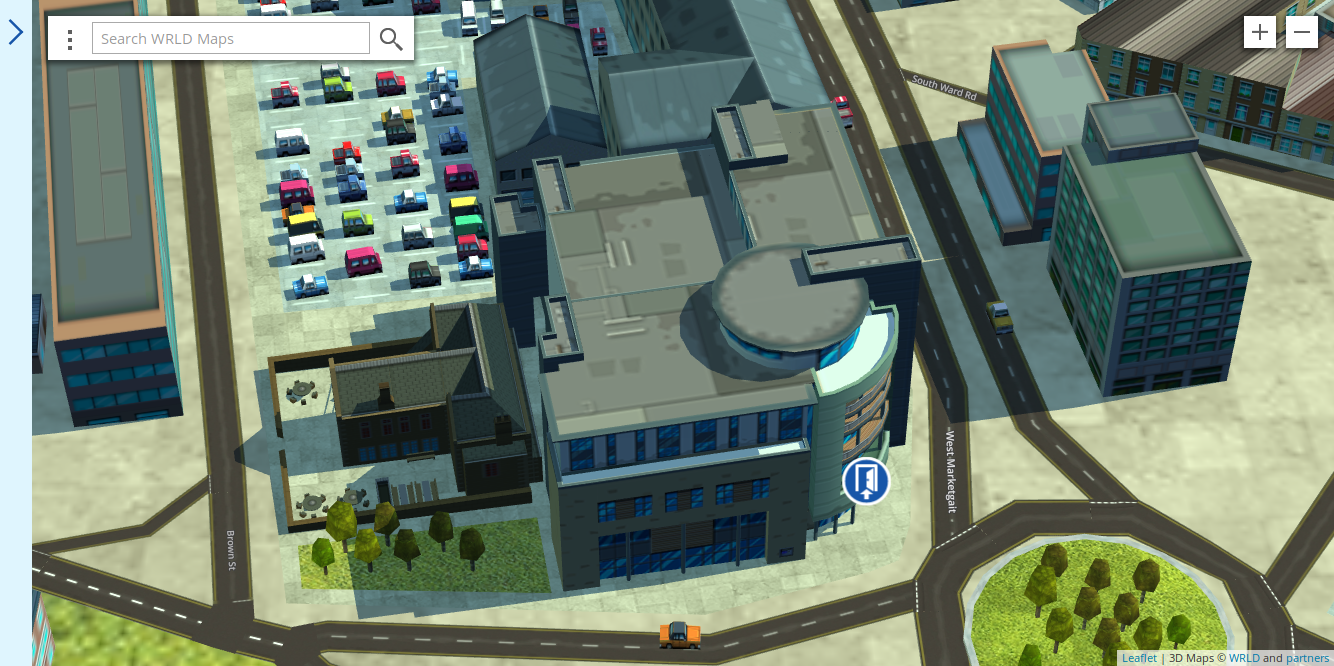
\includegraphics[width=\textwidth]{figures/wrdl_outdoor.png}
        \caption{}
        \label{sfig:wrld_outdoor}
    \end{subfigure}
    \hfill
    \begin{subfigure}{0.49\textwidth}
        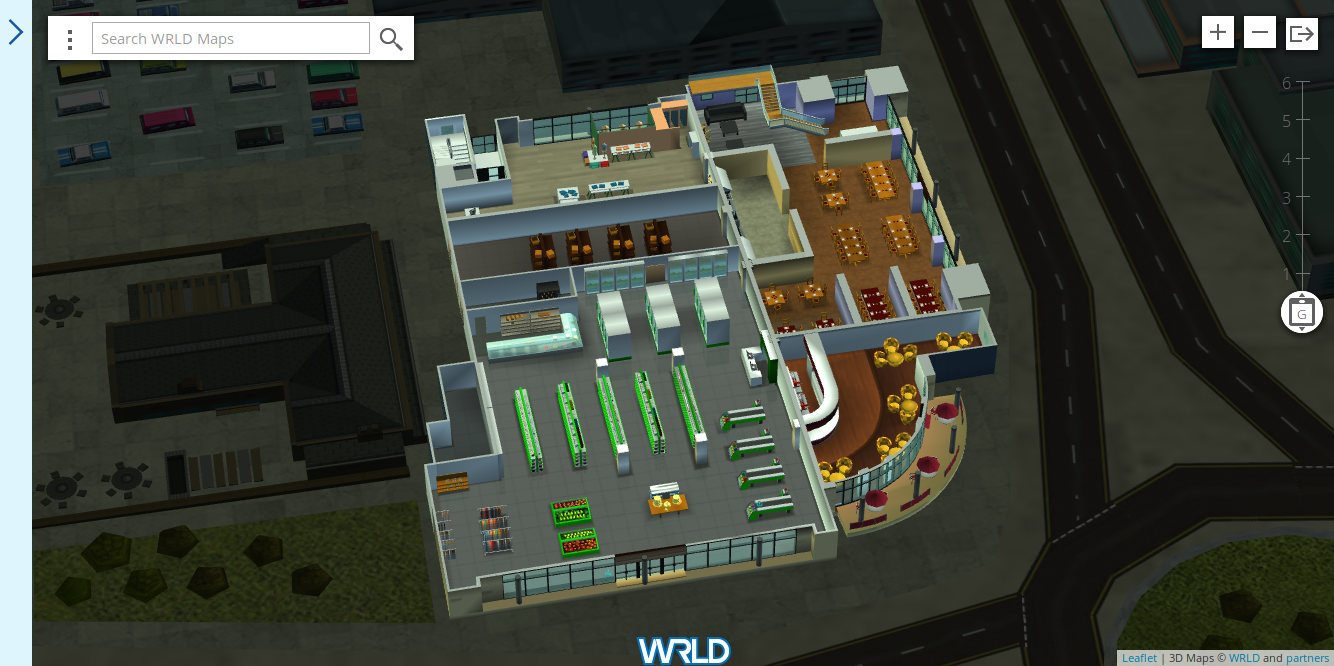
\includegraphics[width=\textwidth]{figures/wrdl_indoor_g.png}
        \caption{}
        \label{sfig:wrld_indoor_g}
    \end{subfigure}
    \newline
    \begin{subfigure}{0.49\textwidth}
        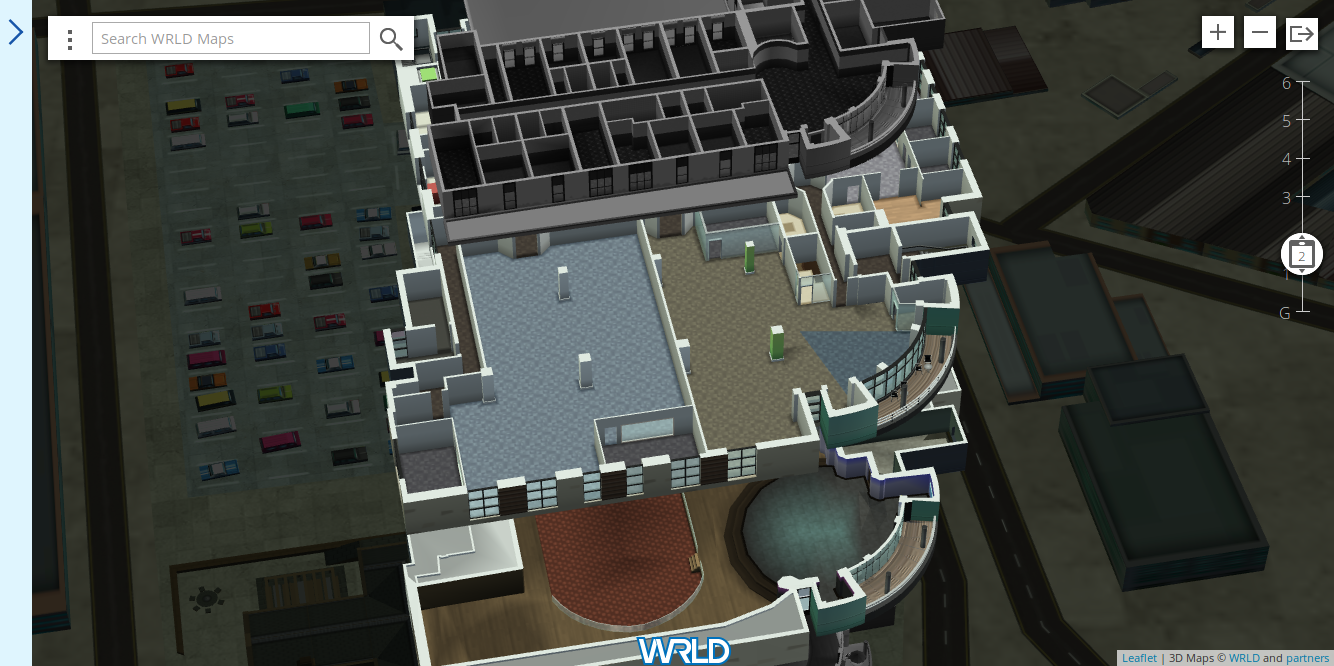
\includegraphics[width=\textwidth]{figures/wrdl_indoor_transition.png}
        \caption{}
        \label{sfig:wrld_indoor_transition}
    \end{subfigure}
    \hfill
    \begin{subfigure}{0.49\textwidth}
        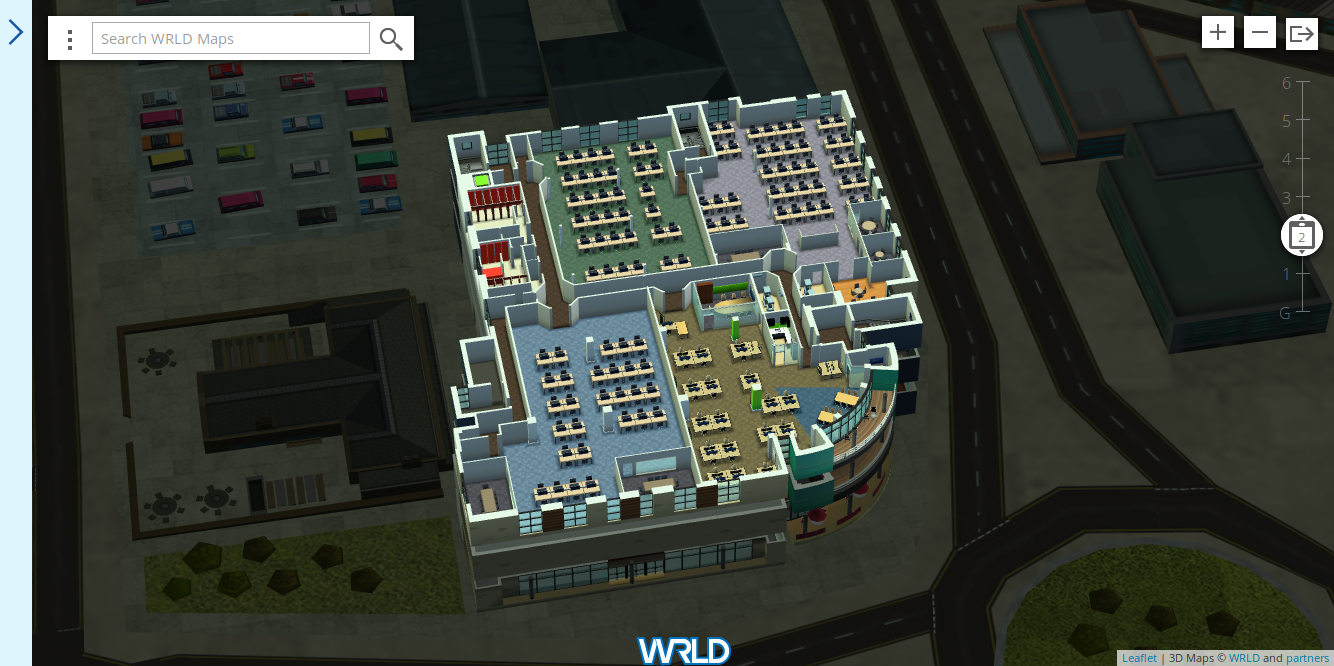
\includegraphics[width=\textwidth]{figures/wrdl_indoor_2.png}
        \caption{}
        \label{sfig:wrld_indoor_2}
    \end{subfigure}
    \caption{Indoor-Funktionalität von WRLD.\@ %
        \textbf{(\subref{sfig:wrld_outdoor})} Das Gebäude ist von außen sichtbar. %
        Über einen Button kann das Gebäude betreten werden. %
        \textbf{(\subref{sfig:wrld_indoor_g})}(\subref{sfig:wrld_indoor_g}) Die Innenansicht des Gebäudes mitsamt Einrichtung wird angezeigt. %
        \textbf{(\subref{sfig:wrld_indoor_transition})} Über einen Slider können die Stockwerke gewechselt werden. %
        \textbf{(\subref{sfig:wrld_indoor_2})} Untenliegende Stockwerke werden vom aktuellen Stockwerk verdeckt.%
    }
    \label{fig:wrld_indoor}
\end{figure}

Die \textbf{zweite} ausprobierte Alternative ist das Mapbox SDK für Unity.
Mapbox bietet sowohl Raster-Tiles (Satellitenbilder) als auch Vektor-Tiles (vektorbasierte Straßen- und Gebäudeumrisse) an.
Es bezieht seine Daten über unterschiedliche Provider, einschließlich OpenStreetMap \autocite{Mapbox2018}.
Sofern die OpenStreetMap-Daten Informationen über die Beschaffenheit der Gebäude liefern, wie z.\,B. die Höhe, können diese Daten für eine 3D-Visualisierung mit Mapbox ausgelesen werden.
Für die Umrisse der Gebäude werden Polygone generiert und entsprechend der Höhe extrudiert.
Da Mapbox keine \emph{explizite} Unterstützung für Indoor-Karten anbietet, müssen diese über einen Umweg eingebunden werden (wie in \cite{Mapbox2018b, Pavani2018, Clarke2017} beschrieben).
Ein georeferenzierter Lageplan des Gebäudes kann auf die Mapbox-Server geladen und in Unity ausgelesen werden.
\autoref{fig:mapbox_unity_mzh_e5_z15} zeigt die 3D-Darstellung eines zuvor erstellten Lageplans.
\begin{figure}[h]
    \centering
    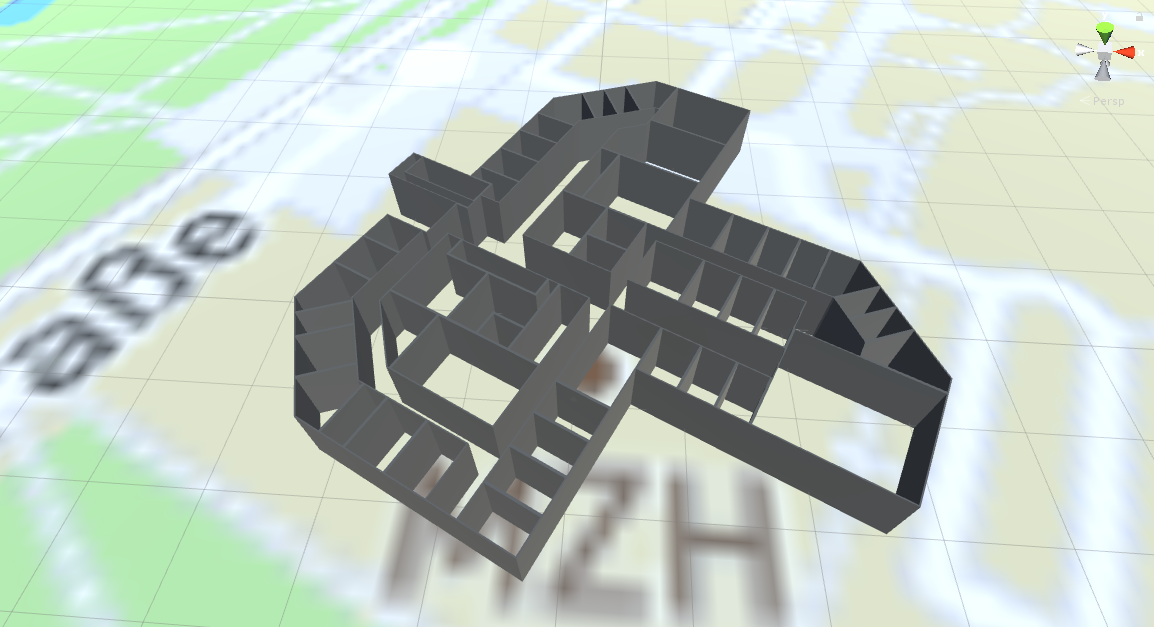
\includegraphics[width=0.65\linewidth]{figures/mapbox_unity_mzh_e5_z15_working}
    \caption{3D-Darstellung des Lageplans des MZH Ebene 5 über das Mapbox Unity Plugin.}
    \label{fig:mapbox_unity_mzh_e5_z15}
\end{figure}
Bei der Verwendung von Mapbox für Gebäudelayouts entstanden visuelle Artefakte (fehlende oder hinzugefügte Wände, Artefaktpolygone) die aus Rundungs- und Präzisionsfehlern resultierten \parencite{Kahyaoglu2017, Mapbox2018c}.
Daher wurde sich gegen einen Ansatz mit Mapbox entschieden.
Für Anwendungen, bei denen eine Megamap für Außenbereiche entworfen werden soll, bietet sich das Mapbox SDK weiterhin an.

\section{Ausblick}
In dieser Arbeit wurde das grundlegende Konzept für die augmentierte Kartenexploration anhand einer Megamap entwickelt.
Die Möglichkeiten für zukünftige Ansätze in MR sind keineswegs abgehandelt.
Sowohl das Konzept als auch der Prototyp sollen der Anstoß für weitere Forschung in diesem Bereich sein.
Da die Idee für die Megamap aus einem Spiel entstammt ist es naheliegend, andere Navigations- und Explorationselemente aus Spielen mit der Megamap zu kombinieren.
Beispielsweise könnte ein MR-HUD eine Minikarte oder eine Kompassleiste zeigen, wenn die Megamap ausgeblendet wird.

Die Probanden wurden zum Ende des Interviews über ihre Meinung für potentielle Anwendungen einer Megamap befragt.
Viele der Probanden konnten sich den Einsatz der Megamap für komplexe, mehrstöckige Gebäude vorstellen, wie z.\,B. in Einkaufszentren oder Flughäfen.
Vor allem in Gebäuden, in denen die Navigation und Exploration in drei Dimensionen stattfindet, sehen sie die Vorteile einer Megamap.
Aber auch die MR-Megamap für den Einsatz im Freien wurde als mögliche Anwendung genannt.
Die Megamap könnte nicht nur einzelne Gebäude, sondern ganze Gebiete anzeigen.
Die dreidimensionalen Gebäude und Strukturen auf der Megamap wären denen der Umgebung nachempfunden, um den mentalen Aufwand beim Wechsel zwischen Karte und Umgebung zu verringern.
Probanden nannten auch eine Kombination aus Megamap und augmentierter Navigation (wie in TCTD) als möglichen Anwendungsfall.

Momentan werden komplexere Anwendungen durch die Möglichkeiten aktueller Mixed-Reality-Technologien beschränkt, vor allem im Freien.
Aber das Interesse seitens der Industrie an Innovation im Bereich Mixed~Reality wird z.\,B. durch die Finanzierung des Magic~Leap Startups in Höhe von ca. 2~Mrd. Dollar \parencite{Machkovech2017} deutlich.
Mit dem Fortschritt der Technologie werden Mixed-Reality-Anwendungen wie die Megamap in Zukunft für den alltäglichen Einsatz möglich sein.

%
\cleardoublepage
